%%
%% This is file `sample-manuscript.tex',
%% generated with the docstrip utility.
%%
%% The original source files were:
%%
%% samples.dtx  (with options: `manuscript')
%%
%% IMPORTANT NOTICE:
%%
%% For the copyright see the source file.
%%
%% Any modified versions of this file must be renamed
%% with new filenames distinct from sample-manuscript.tex.
%%
%% For distribution of the original source see the terms
%% for copying and modification in the file samples.dtx.
%%
%% This generated file may be distributed as long as the
%% original source files, as listed above, are part of the
%% same distribution. (The sources need not necessarily be
%% in the same archive or directory.)
%%
%% Commands for TeXCount
%TC:macro \cite [option:text,text]
%TC:macro \citep [option:text,text]
%TC:macro \citet [option:text,text]
%TC:envir table 0 1
%TC:envir table* 0 1
%TC:envir tabular [ignore] word
%TC:envir displaymath 0 word
%TC:envir math 0 word
%TC:envir comment 0 0
%%
%%
%% The first command in your LaTeX source must be the \documentclass command.
\documentclass[manuscript,screen,natbib=false]{acmart}
% [review]
\usepackage{multirow}

\usepackage[style=acmnumeric]{biblatex}
\addbibresource{main.bib}


%%
%% \BibTeX command to typeset BibTeX logo in the docs
\AtBeginDocument{%
  \providecommand\BibTeX{{%
    \normalfont B\kern-0.5em{\scshape i\kern-0.25em b}\kern-0.8em\TeX}}}

%% Rights management information.  This information is sent to you
%% when you complete the rights form.  These commands have SAMPLE
%% values in them; it is your responsibility as an author to replace
%% the commands and values with those provided to you when you
%% complete the rights form.
% \setcopyright{acmcopyright}
\copyrightyear{2022}
\acmYear{2022}
% \acmDOI{XXXXXXX.XXXXXXX}

%% These commands are for a PROCEEDINGS abstract or paper.
% \acmConference[Conference acronym 'XX]{Make sure to enter the correct
%   conference title from your rights confirmation emai}{June 03--05,
%   2018}{Woodstock, NY}
% \acmPrice{15.00}
% \acmISBN{978-1-4503-XXXX-X/18/06}


%%
%% Submission ID.
%% Use this when submitting an article to a sponsored event. You'll
%% receive a unique submission ID from the organizers
%% of the event, and this ID should be used as the parameter to this command.
%%\acmSubmissionID{123-A56-BU3}

%%
%% For managing citations, it is recommended to use bibliography
%% files in BibTeX format.
%%
%% You can then either use BibTeX with the ACM-Reference-Format style,
%% or BibLaTeX with the acmnumeric or acmauthoryear sytles, that include
%% support for advanced citation of software artefact from the
%% biblatex-software package, also separately available on CTAN.
%%
%% Look at the sample-*-biblatex.tex files for templates showcasing
%% the biblatex styles.
%%

%%
%% The majority of ACM publications use numbered citations and
%% references.  The command \citestyle{authoryear} switches to the
%% "author year" style.
%%
%% If you are preparing content for an event
%% sponsored by ACM SIGGRAPH, you must use the "author year" style of
%% citations and references.
%% Uncommenting
%% the next command will enable that style.
%%\citestyle{acmauthoryear}

%%
%% end of the preamble, start of the body of the document source.
\begin{document}

%%
%% The "title" command has an optional parameter,
%% allowing the author to define a "short title" to be used in page headers.
\title{A Review on Creating a Performance Adaptive Generalized Abstractive text Summarization using Optimized Transformers}

%%
%% The "author" command and its associated commands are used to define
%% the authors and their affiliations.
%% Of note is the shared affiliation of the first two authors, and the
%% "authornote" and "authornotemark" commands
%% used to denote shared contribution to the research.
\author{Nazhim Kalam}
% \authornote{Both authors contributed equally to this research.}
\email{nazhimkalam@gmail.com}
\orcid{0009-0005-9507-601X}
% \author{G.K.M. Tobin}
% \authornotemark[1]
% \email{webmaster@marysville-ohio.com}
\affiliation{%
  \institution{University of Westminster}
  \streetaddress{309 Regent St.}
  \city{London}
%   \state{Ohio}
  \country{UK}
%   \postcode{43017-6221}
}

\author{Torin Wirasingha}
\affiliation{%
  \institution{Informatics Institute of Technology}
  \streetaddress{57 Ramakrishna Rd}
  \city{Colombo 06}
  \country{Sri Lanka}}
\email{torin.w@iit.ac.lk}

%%
%% By default, the full list of authors will be used in the page
%% headers. Often, this list is too long, and will overlap
%% other information printed in the page headers. This command allows
%% the author to define a more concise list
%% of authors' names for this purpose.
% \renewcommand{\shortauthors}{Trovato and Tobin, et al.}

%%
%% The abstract is a short summary of the work to be presented in the
%% article.
\begin{abstract}
Abstractive text summarization systems have been integrated with various applications in the world to perform text summarization, and it's nothing new to the field. However, with prior research it found that in the domain of movies the need for performance improvement is required using the latest approaches than the current traditional ML & DL methods, movie review summarization plays a major role in helping users to make better decisions by matching their interest with the reviews of the movie, this saves a lot of time and also improves businesses in their sales.

In 2017 researchers from Google Brain introduced NLP Transformers, which is the latest approach to solving NLP problems, and it's increasingly been known and used nowadays over traditional ML & DL approaches like using basic LSTM, and RNN approaches. The author explored ways in which to get an optimal solution using Transformer for abstractive text summarization and yet making a generalized solution that can be adapted with respect to any domain (be it hotels, movies, restaurants) and increase its performance as the system gets used over time.

This paper is a review of the approach taken to explore and construct a performance-adaptive generalized abstractive text summarizer using optimized transformers. The approach taken to optimize transformers will be discussed in this review.
\end{abstract}

%%
%% The code below is generated by the tool at http://dl.acm.org/ccs.cfm.
%% Please copy and paste the code instead of the example below.
%%
\begin{CCSXML}
<ccs2012>
<concept>
<concept_id>10002951.10003317.10003347.10003350</concept_id>
<concept_desc>Computing methodologies</concept_desc>
<concept_significance>500</concept_significance>
</concept>
<concept>
<concept_id>10003120.10003130.10003131.10003270</concept_id>
<concept_desc>Artificial intelligence</concept_desc>
<concept_significance>500</concept_significance>
</concept>
<concept>
<concept_id>10002951.10003317.10003338</concept_id>
<concept_desc>Natural language processing</concept_desc>
<concept_significance>300</concept_significance>
</concept>
<concept>
<concept_id>10002951.10003227.10003351</concept_id>
<concept_desc>Natural language generation</concept_desc>
<concept_significance>300</concept_significance>
</concept>
</ccs2012>
\end{CCSXML}

\ccsdesc[500]{Computing methodologies}
\ccsdesc[500]{Artificial intelligence}
\ccsdesc[300]{Natural language processing}
\ccsdesc[300]{Natural language generation}

%%
%% Keywords. The author(s) should pick words that accurately describe
%% the work being presented. Separate the keywords with commas.
\keywords{Natural Language Processing (NLP), Machine Learning (ML), Deep Learning (DL), Recall-Oriented Understudy for Gisting Evaluation (ROUGE), Inductive logic programming (ILP)}

%%
%% This command processes the author and affiliation and title
%% information and builds the first part of the formatted document.
\maketitle

% 
% This is how citation is added '\cite{naumov_deep_2019}'
% 

\section{Introduction}
A growing number of websites, like Amazon and the Internet Movie Database (IMBD), a website for movie reviews, allow users to publish reviews for things they are interested in, along with the growth of Web 2.0, where user interaction is prioritized. \cite{khan_gul_zareei_biswal_zeb_naeem_saeed_salim_2020}

Online movie reviews are evolving into an important information source for users, with the continuous increase in data on the web \cite{m_mehla_2019}. However, online users post a significant number of movies reviews every day, hence making it difficult for them to manually summarize the reviews and determine their interest in the film. One of the challenging problems in natural language processing is mining and summarizing movie reviews. \cite{khan_gul_zareei_biswal_zeb_naeem_saeed_salim_2020}.
% You must have at least 2 lines in the paragraph with the drop letter
% (should never be an issue)

Text summary assist users or business decision-makers by compiling and analyzing a significant number of online reviews. \cite{alsaqer_sasi_2017}

These days, the majority of people research a film's reviews before selecting or watching it on any platform, such Netflix or Amazon Prime, but we also come across conflicting reviews that can be either good or bad. While most reviews are detailed and require a significant amount of time to review, this develops a problem where users aren't able to make quicker decisions. Therefore, by summarizing the review makes it easier and faster for users to make decisions. This can also help streaming services like Netflix quickly discover the viewing habits or preferences of their users \cite{dashtipour_gogate_adeel_larijani_hussain_2021}

\section{Business corporate advantage}
It is also known that it costs at least five times as much time and money to acquire a new customer as it does to keep an existing one, so it is important to learn how to foster customer loyalty to the brand, business, or service that is being offered. Customer satisfaction is essential to the survival of corporate industries. Understanding client expectations through their feedback or reviews helps business industries grow and fix faults \cite{pizam_ellis_1999}

On the other hand, companies like Netflix or Amazon Prime can use movie summaries to help users understand their watching pattern or their interest. Likewise, movie-related industries need to allow customers to quickly scan the summary and quickly decide whether they should be watching it or not \cite{khan_gul_zareei_biswal_zeb_naeem_saeed_salim_2020}

\section{Text summarization and techniques}
With the massive accumulation of information/data on the internet nowadays, it is extremely difficult to extract relevant information from a large number of textual documents. The goal of text summarizing is to provide a condensed yet meaningful version of lengthy textual content \cite{shi_keneshloo_ramakrishnan_reddy_2020}
We all know that text summarization has several uses in a variety of internet-based fields, including search engines that are used for querying and e-commerce sites that utilize sentiment analysis to determine client satisfaction with items \cite{etemad_abidi_chhabra_2021}

However, in the movie industry, consumers may utilize text summarization to simplify customer reviews of movies, which are often lengthy and time-consuming to read. This enables users to make better decisions when they decide whether or not to watch a certain movie \cite{khan_gul_zareei_biswal_zeb_naeem_saeed_salim_2020}

Generally, text summarization is classified into two which are; abstractive text summarization and extractive text summarization, however, the approach for creating a hybrid model for text summarization is possible \cite{alsaqer_sasi_2017}. The abstractive text summarization technique aims to produce sentences on its own and then uses them to provide a coherent summary. Therefore, the summary's content will vary from the original context yet still convey the same idea \cite{duseja_2020}. Additionally, it is well-recognized that a strong abstractive summary encompasses the input's key details and is linguistically fluent \cite{zhang_xu_wang_2019}.

The extractive text summarizing method focuses on picking out key phrases or groups of phrases from the original input content and combining them to produce a concise yet insightful text summary. It is determined which sentences should be included as parts of the summary based on the statistical and linguistic characteristics of the sentences \cite{gupta_lehal_2010}
A hybrid system is one that combines various strategies to produce a single system. However, hybrid text summarizing systems do exist, for instance, using a combination of extractive and abstractive summarization can be utilized to generate a hybrid system that uses encoder-decoders \cite{kirmani_manzoor}

\section{NLP with deep learning}
NLP is a method for computers to intelligently and effectively analyze, comprehend, and derive meaning from human language, as opposed to other approaches that only focus on the interactions between human language and computers. Deep learning techniques are increasingly being used in the field of AI compared to traditional machine learning approaches due to their success rates in handling difficult high-computing learning tasks \cite{lopez_kalita_2017}

In today's NLP, machine learning is prominent, but for the most part, it only involves numerically optimizing the weights of characteristics and representations that have been created by humans. Deep learning aims to investigate how computers can utilize data to create features and representations suitable for challenging interpretation tasks \cite{socher_bengio_manning}.

\section{NLP transformer models}

Open-source library Transformers contains modern transformer architectures that have been thoroughly developed and are integrated by a common API. Pretraining has enabled the efficient use of this capacity for a wide range of activities, and these designs have permitted the construction of higher-capacity models. Transformers are designed to be easy for practitioners, expandable for researchers, and quick and reliable in industrial deployments \cite{wolf__2020}

It has been demonstrated that the modern generation of pre-trained language models based on transformers is rather competent at identifying syntactic signals like noun modifiers, possessive pronouns, prepositions, or co-referents, as well as semantic cues like entities and relations \cite{brasoveanu_andonie_2020}

Hugging Face Hub offers a variety of transformer designs, including BERT, GPT2, T5, PEGASUS, and many others. The figure below represents the daily average for unique downloads of the pretrained transformer model architectures between Oct 2019 to May 2020 \cite{wolf__2020}

\begin{figure}[h]
\centering
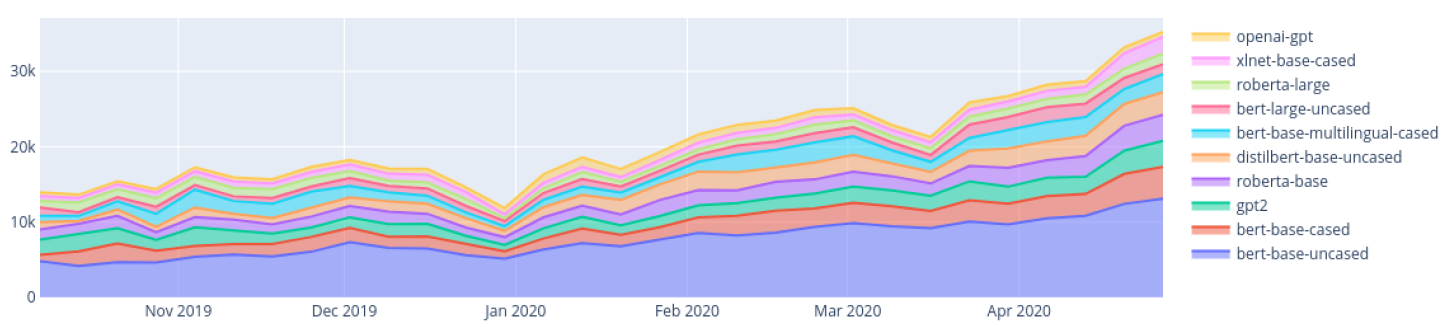
\includegraphics[width=\textwidth]{images/LR-Transformer Models Popularity.png}
\caption{Transformer Architecture Downloads Rate \cite{wolf__2020}}
\label{fig:transformer-architecture-model-popularity}
\end{figure}

\cite{etemad_abidi_chhabra_2021} research compares various other researchers approaches taken in order to perform abstractive text summarization, these techniques includes the use of transformers and other neural network approaches such as CNN and LSTM RNN networks. The research comparison table below only includes the approaches of transformers used taken abstractive text summarization.

\section{Automated hyperparameter model tuning}

Finding the ideal collection of parameter values to train an algorithm using in order to build a model relevant to the dataset is known as hyperparameter tuning \cite{liu_wang_2021}. The calculation of the performance improvement that may be obtained by changing the value of each of the considered hyperparameters from the original value to the value indicated in the target configuration set by the tuning strategy is where hyperparameters make the biggest contribution to improving algorithm performance \cite{joy_selvan_2022}

There are several hyperparameters that play a significant role in performance enhancement; however, not all of the parameters do so; just a select handful do, for example, learning rate, weight decay, number of epochs, batch size, and warm up ratio. As a result, giving critical hyperparameters a higher priority is crucial \cite{engdahl_2008}

Automated framework tools, such as Optuna, an open-source framework for hyperparameter optimization built on the Python programming language, does hyperparameter tweaking. The application of numerous hyperparameter optimization techniques, including Grid Search, Random Search, TPE, and CMA-ES algorithms, was made easier by this framework \cite{joy_selvan_2022}

\section{Model Generalization}

Generalization now plays a significant part in resolving issues in numerous fields that are linked to the same issue. The capacity of a model to generalize to new, previously unobserved data that comes from the same distribution as the model's original data is known as generalization \cite{semantic_scholar} 

Generalization is a useful strategy for starting with the foundation and improving or specializing in one's field as more unseen domain data becomes available. Therefore, the generalized solution will be able to adapt to even unseen domain data, making this solution to solve a common problem in multiple domain \cite{Zhou_2021}

\begin{figure}[h]
\centering
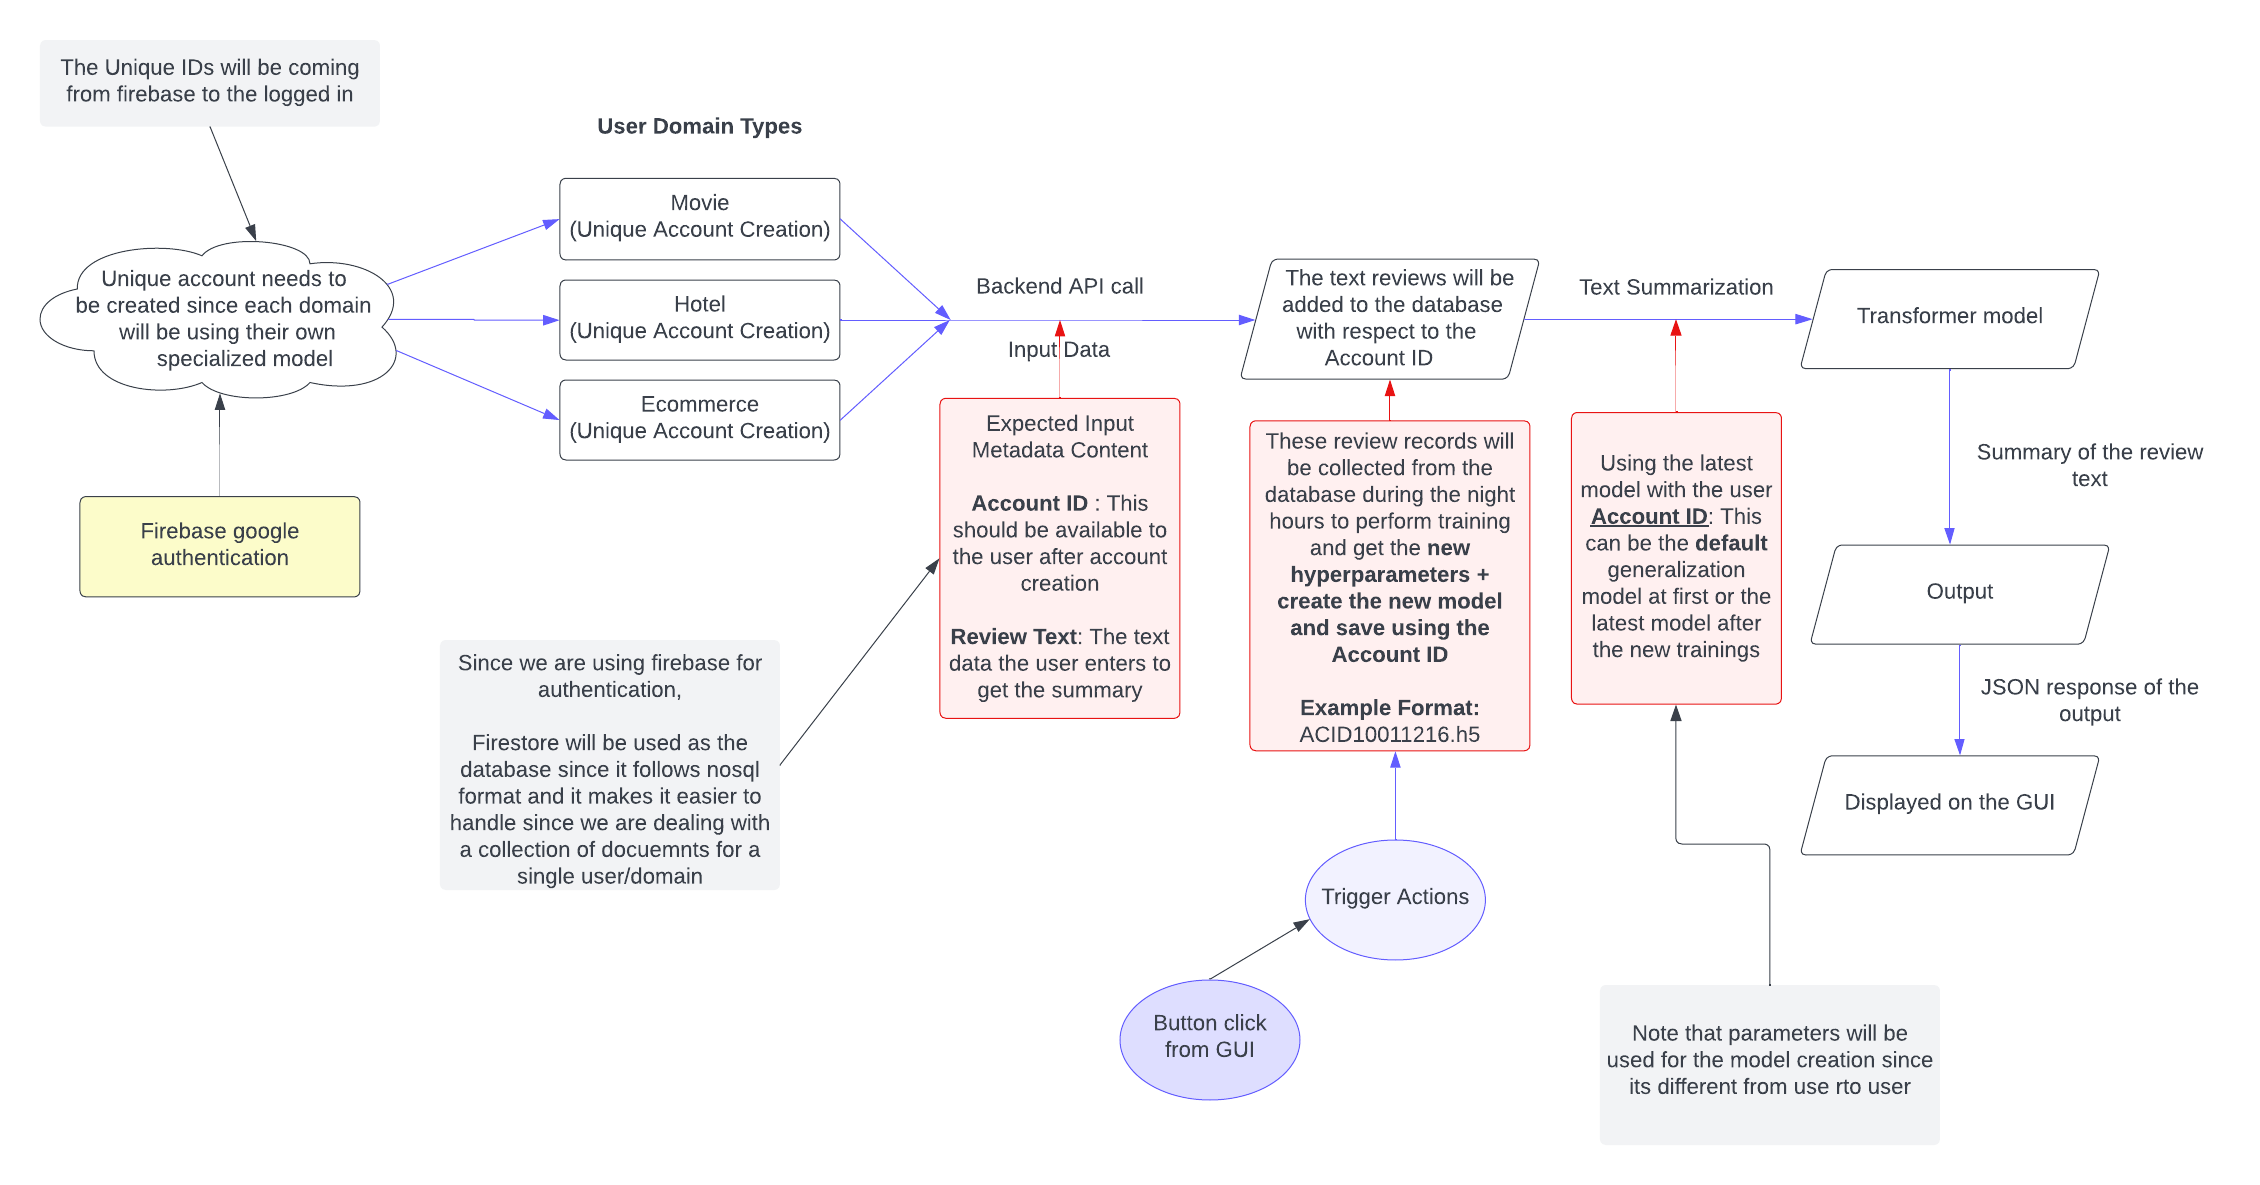
\includegraphics[width=\textwidth]{images/LR-Proposed Archtecture.png}
\caption{Proposed Generalized Abstractive Summarization System Process Flow \textit{(self-composed)}}
\label{fig:model-generalization-for-abstractive-text-summarization}
\end{figure}

\section{Algorithmic approaches for Text Summarization}
The study of \cite{khan_gul_zareei_biswal_zeb_naeem_saeed_salim_2020} starts by first focusing on feature extraction, then transforming reviews into vector spaces, and applying the Naive Bayes machine learning method for review classification utilizing an undirected weighted graph-based ranking algorithm to rank score for each review phrase in graph and then, in order to construct the extractive summary, the highest scoring sentences are selected. However, the author has limited the use of sophisticated deep learning algorithms to improve performance by solely using standard machine learning approaches to tackle the problem.

\cite{brasoveanu_andonie_2020} research made use of seq2seq model for text summarization along with the attention mechanism for improved accuracy and the Concept net Number batch word embedding model, which is superior than Glove. Utilizing a 1D convolutional layer, a max pooling layer, an LSTM layer, and finally a fully connected layer at the very end. However, the author's use of generic deep learning algorithms to handle this problem introduces a new constraint that prevents performance from being improved using the most recent deep learning strategy for NLP-related problems, transformers.

The research of \cite{mukherjee_peruri_vishnu_goyal_bhattacharya_ganguly_2020} liked mentioned earlier is an extractive method text summarization based on integer linear programming (ILP [Unsupervised method]) to choose an informative subset of opinions centered on the identified aspects. Utilize ROUGE-based criteria to assess and contrast the summaries and get competitive outcomes. Since the dataset is also constrained, extractive summaries could not be particularly insightful; thus, utilizing an abstractive technique might produce superior results, despite the dataset's constrained size.

The study of \cite{etemad_abidi_chhabra_2021} focus of the authors' study is utilizing the encoder-decoder model with the attention layer to produce text summaries with good syntax and no repeated words. the creation of an encoder-decoder model with gated recurrent units and training it to provide an abstract summary of a piece of writing. Although the author employed deep learning, its application in production 

\section{Usage of transformers}
\cite{gupta_lehal_2010} research employed pretrained models such Pipeline BART, BART modified, T5, and PEGASUS to deal with text summarization as a part of the comparison study done. The ROUGE Scores were used as the evaluation measures. During the experiments, the author employed transformer designs; however, the hyperparameters used were default and might be tuned for a better performance. The constraints consist of concentrating on developing more reliable models that can further expand the method to produce summaries of varying length and applicable for multi-document summarization.

\cite{etemad_abidi_chhabra_2021} The author explores with deep learning methods in the broad text summarization domain to determine which method—among a collection that includes RNN, CNN, and Transformers—performs best. The author also considers metrics for model evaluations including BLEU and ROUGE, despite using sophisticated deep learning algorithms, the author was unable to undertake hyperparameter tuning to improve the method and obtain a better outcome.

\section{Machine Learning text summarization techniques}
\cite{boorugu_ramesh_2020} points out a previous research where a system was built that uses a hybrid classifier approach with machine learning algorithm combination of SVM and Naïve Bayes in sync with fuzzy logic and they also concluded that with the increase in the classifier count the accuracy can also be increased. They also made use of supervised ML algorithms such as KNN for the classification of the reviews which then combining appropriate words for identifying the features of the product.

\cite{khan_gul_zareei_biswal_zeb_naeem_saeed_salim_2020} proposed system was for the movies domain using the customer reviews, the author broke down proposed methodology into segments of which is preprocessing, feature extraction, review classification and finally review summarization. The Nave Bayes (NB) classification method, which is regarded as a robust classifier and may achieve greater accuracy, was used to categorize the reviews from negative to positive using supervised ML classification technique, It is clear that an extractive summarization approach was used because the text summarization phase was completed in several stages, starting with the creation of a graph from classified reviews, followed by the ranking of graph nodes and the selection of the top rank sentences for the summary generation.

Initially, these machine learning methodologies were given a lot of significance, but as time has progressed on, new technologies and techniques have emerged that can utilize deep learning techniques like RNN, CNN, etc. to perform better.

\section{Deep Learning text summarization techniques}
Numerous studies have been conducted on deep learning methods for abstractive text summarization, such as with the usage of CNN, LSTM-CNN, Convolutional Seq2Seq, Sequence to Sequence RNN, Convolutional Sequence to Sequence, Transformers, T5, BART, BERT etc.… which were trained on a general dataset such as from Gigaword, DUC 2002, DUC 2004, CNN Daily Mail, DUC, Xsum, Newsroom such datasets, in order to get an evaluation comparison on which outperforms the rest and eventually the T5 Transformer outperformed the rest of the other techniques in the case of abstractive text summarization \cite{etemad_abidi_chhabra_2021}

\cite{shi_keneshloo_ramakrishnan_reddy_2020} has conducted a thorough analysis of latest developments in seq2seq models for the task of abstractive text summarizing. The author's analysis includes a full review of several distinct seq2seq models for abstractive summarization.

Out of which transformers are the advanced deep learning approach for text summarization which is an encoder-decoder model with attention layer which helps it to generate better results than a traditional simple RNN architecture \cite{etemad_abidi_chhabra_2021}

\section{Available Datasets for generalized text summarization}
There are two datasets that the author will be exploring throughout the development of this project. One of which is the Amazon movie reviews dataset from Stanford University Education, which contains data within the span period of more than 10 years including 8 million review data records \cite{mcauley_leskovec_2013}

This dataset will be used to test out the solution for the problem domain which is abstractive text summarization for movies. Given that the author is able to create the solution for the domain of movies then, the author then plans to generalize the solution using another dataset named as Gigaword which is from TensorFlow datasets which was used previously for creating generalized content for text summarization \cite{kouris_alexandridis_stafylopatis_2019}

\section{Preprocessing techniques used in text summarization.}
Text preprocessing is very important when it comes to dealing with text related data. In earlier studies, a variety of text preprocessing approaches were utilized for text summarization. 

Sentence segmentation is a fundamental step in NLP applications including IR, machine translation, semantic role labeling, and summarization. It is the process of identifying boundaries within a document that divides the document's text into sentences, typically from a strong point of punctuation like (full stop, explanation mark, question mark, etc.), Tokenization and stop words removal will then be performed. Tokenization will be carried out by the tokenizer program to split the sentences into distinct words by splitting them at whitespaces such as blanks, tabs, and any strong punctuation. Stop word removal is also used to remove frequently used words in the document such as "I," "an," and "a" because these words carry little meaning and are best removed from the document \cite{khan_gul_zareei_biswal_zeb_naeem_saeed_salim_2020}

Other researchers have incorporated a variety of other techniques, including noise removal, which eliminates unnecessary text from the input document, such as the header and footer, and named entity recognition (NER), which recognizes words in the input text as names of things like people, places, and things, among others \cite{barna_heickal_2022}

Datasets may also contain unwanted records, null records, or redundant records that are absolutely useless. These records or rows with null values are eliminated, unnecessary HTML tags and URL links are also filtered off from the text as a part of text preprocessing. Contraction mapping is crucial and this will be handling which are converting short word formats into longer such as “aren’t” into “are not”. Converting the entire text content into a single case most preferably to lowercase, therefore further character filtration would become very simpler \cite{etemad_abidi_chhabra_2021}

\section{Evaluation techniques}
A machine learning model's performance, as well as its advantages and disadvantages, are understood through the process of model evaluation, which employs many evaluation measures. During the early stages of research, it's critical to evaluate models to determine their efficiency.
The table below shows the available measure and the metrics that can been used to quantitatively evaluate the text summarization system. 

\begin{table}[h]
\caption{Evaluation techniques for abstractive text summarization}
\label{tab:evaluation-techniques-table}
\centering
\begin{tabular}{|l|p{0.5\linewidth}|p{0.21\linewidth}|}
\hline
Measure & Description & Objective Orientation \\
\hline
ROUGE & Measures are made by comparison between an automatically generated summary/translation against a group of reference summaries (generally human created summaries) & \multirow{2}{=}{Positively oriented. Higher, the better.} \\ 
\cline{1-2}
BLEU & measures the precision (as to how much words in the generated summaries appeared in the human generated summaries) & \\
\hline 
\end{tabular}
\end{table}

ROUGE also known as Recall-Oriented Understudy for Gisting Evaluation. Measures are made by comparison between an automatically generated summary/translation against a group of reference summaries (generally human created summaries) \cite{lin_2004}. ROUGE measures the recall, (according to how frequently the terms from the summaries created by humans appeared in those computers - generated.)

BLEU also known as Bilingual Evaluation Understudy is a metric used for evaluation for the quality of machine generated text by comparing it with a reference text that is supposed to be generated. \cite{steinberger_ježek}. BLEU measures the precision (as to how much words in the generated summaries appeared in the human generated summaries)

\section{Conclusion}
In this review, the author has pointed out the reasons for the need for the need of performance increase for abstractive review summarization and how NLP transformers can be used as the solution.

Moreover the author also discusses how and why the solution is generalized along with the ways in making using automated hyperparameter tools and model retraining, evaluations metrics is also included by the author along with their objected orientations.

%%
%% The acknowledgments section is defined using the "acks" environment
%% (and NOT an unnumbered section). This ensures the proper
%% identification of the section in the article metadata, and the
%% consistent spelling of the heading.
% \begin{acks}
% To Robert, for the bagels and explaining CMYK and color spaces.
% \end{acks}

%%
%% The next two lines define the bibliography style to be used, and
%% the bibliography file.
% \bibliographystyle{ACM-Reference-Format}
% \bibliography{sample-base}
\printbibliography


%%
%% If your work has an appendix, this is the place to put it.
% \appendix

% \section{Research Methods}

% \subsection{Part One}

% Lorem ipsum dolor sit amet, consectetur adipiscing elit. Morbi
% malesuada, quam in pulvinar varius, metus nunc fermentum urna, id
% sollicitudin purus odio sit amet enim. Aliquam ullamcorper eu ipsum
% vel mollis. Curabitur quis dictum nisl. Phasellus vel semper risus, et
% lacinia dolor. Integer ultricies commodo sem nec semper.

% \subsection{Part Two}

% Etiam commodo feugiat nisl pulvinar pellentesque. Etiam auctor sodales
% ligula, non varius nibh pulvinar semper. Suspendisse nec lectus non
% ipsum convallis congue hendrerit vitae sapien. Donec at laoreet
% eros. Vivamus non purus placerat, scelerisque diam eu, cursus
% ante. Etiam aliquam tortor auctor efficitur mattis.

% \section{Online Resources}

% Nam id fermentum dui. Suspendisse sagittis tortor a nulla mollis, in
% pulvinar ex pretium. Sed interdum orci quis metus euismod, et sagittis
% enim maximus. Vestibulum gravida massa ut felis suscipit
% congue. Quisque mattis elit a risus ultrices commodo venenatis eget
% dui. Etiam sagittis eleifend elementum.

% Nam interdum magna at lectus dignissim, ac dignissim lorem
% rhoncus. Maecenas eu arcu ac neque placerat aliquam. Nunc pulvinar
% massa et mattis lacinia.

\end{document}
\endinput
%%
%% End of file `sample-manuscript.tex'.
